\documentclass[11pt,a4paper]{article}

\usepackage{fontspec}
\usepackage[main=english]{babel}
\babelfont{rm}{Latin Modern Roman}
\usepackage{amsmath,amssymb,amsthm}
\usepackage{booktabs}
\usepackage{graphicx}
\usepackage{geometry}
\usepackage{hyperref}
\usepackage{enumitem}
\usepackage{verbatim}

\newcommand{\orcid}[1]{\href{https://orcid.org/#1}{\texttt{#1}}}

\geometry{margin=2.4cm}
\hypersetup{
  colorlinks=true,
  linkcolor=blue,
  citecolor=blue,
  urlcolor=blue
}

\newtheorem{proposition}{Proposition}
\newtheorem{lemma}{Lemma}
\newtheorem{definition}{Definition}

\title{Hadamard-Based Rejection Sampling for Fair Dice:\\
A Low-Depth Quantum Circuit Model for Tabletop Games}
\author{Önder Öztürk}
\date{\today}

\begin{document}
\maketitle

{\footnotesize
\noindent
Information Technology Department, Rectorate, Kütahya Health Sciences University, Türkiye \\[0.1em]
\orcid{0000-0001-6460-9497}
}

\begin{abstract}
We present a practical method for producing mathematically fair six-sided dice rolls from quantum measurements. Each die is encoded with three qubits. Applying $H^{\otimes 3}$ to the all-zero state produces a uniform superposition over eight basis states. By rejecting the outcomes 0 and 7 and conditioning on the valid set $\{1,\dots,6\}$, the resulting distribution is exactly uniform ($1/6$ per face). For two dice (as required by backgammon and its variants such as Tavla), the construction extends to a six-qubit product circuit $H^{\otimes 6}$ whose marginals remain independent. The same circuit is exposed through a thin HTTP service that can dispatch to either the Qiskit Aer simulator or IBM Quantum hardware; the game engine consumes only the final classical values together with a provenance/fallback flag. We prove uniformity via elementary conditional probability, demonstrate the bias introduced by the common modulo mapping, and report reproducible (seeded) Aer experiments ($N=50{,}000$ valid rolls) whose marginal and $6\times 6$ joint face distributions are consistent with the predicted uniform law (marginal $\chi^2=10.1$ on $5$ d.o.f., $p=0.07$; joint $\chi^2=26.8$ on $35$ d.o.f., $p=0.84$). Because the Aer simulator performs ideal Born sampling, these experiments validate the sampling pipeline rather than the abstract fairness guarantee, which is already exact. A preliminary single-backend run on real hardware (IBM \texttt{ibm\_marrakesh}, $4000$ shots) exhibits the expected percent-level noise bias (post-rejection $\mathrm{TVD}=0.018$ from uniform); a systematic multi-backend characterisation is left to future work. The approach uses a single layer of Hadamard gates and incurs negligible rejection overhead, making it suitable for low-latency integration in consumer games while cleanly separating quantum sampling from classical game logic.
\end{abstract}

\noindent\textbf{Keywords:} quantum random number generation, rejection sampling, Hadamard circuit, fair dice, Qiskit, backgammon, tabletop games

\section{Introduction}

Fair random number generation is fundamental to the integrity of dice-driven games. In backgammon and its regional variants (collectively ``Tavla''), the joint outcome of two independent six-sided dice directly determines the legal move set. Even small biases in the dice distribution can, over thousands of games, produce measurable advantages for one player or strategy class.

Classical pseudorandom generators (PRNGs) or operating-system entropy sources are adequate for most entertainment software. Nevertheless, there is growing interest in \emph{verifiable} or \emph{externally auditable} randomness, especially in online or blockchain-adjacent gaming, educational demonstrations of quantum computing, and marketing of ``genuinely quantum'' experiences. Cloud-accessible quantum processors~\cite{ibmquantum2024} now make it feasible to obtain measurement samples from explicitly constructed quantum circuits and to expose them through ordinary web APIs.

A naïve approach—prepare $n$ qubits in uniform superposition with $H^{\otimes n}$ and reduce the resulting integer modulo 6—introduces a well-known structural bias: certain faces receive twice the probability of others. We instead adopt \emph{rejection sampling}: the two forbidden outcomes are discarded and the conditional distribution over the remaining six is exactly uniform. The construction is textbook quantum mechanics (uniform superposition) combined with elementary probability, yet it yields a clean, testable, and low-depth implementation that has seen surprisingly little rigorous treatment in the quantum-gaming literature.

Our contributions are:
\begin{enumerate}[label=\arabic*.]
  \item A three-qubit circuit plus rejection rule that realises an exactly fair six-sided die, together with the corresponding two-die product construction (Section~\ref{sec:single}--\ref{sec:two}).
  \item An explicit proof that the conditional distribution is uniform and a side-by-side comparison with the biased modulo mapping (Section~\ref{sec:rejection}).
  \item A production-grade service architecture that preserves the identical mathematical contract on both simulator and real hardware while providing transparent fallback (Section~\ref{sec:arch}).
  \item Large-scale experimental validation on the Qiskit Aer simulator, including $\chi^2$ goodness-of-fit tests, total-variation distances, and empirical confirmation of the per-shot acceptance probability (Section~\ref{sec:exp}).
\end{enumerate}

Related work includes the well-known IBM ``Truly Quantum Dice'' demonstration~\cite{ibmq2024dice}, the quantum random-number-generation surveys of Herrero-Collantes and Garcia-Escartin~\cite{herrero2023quantumrng} and Ma et al.~\cite{ma2016quantum}, and the circuit construction of Orts et al.~\cite{orts2023quantum} for sampling integers inside an arbitrary interval---of which our concrete $d=6$ rule is a special case. Quantum games have previously been realised on a photonic one-way quantum computer~\cite{prevedel2007experimental} and on IBM-Q~\cite{galas2020quantum}. Classical treatments of unbiased sampling from biased sources date back to von Neumann~\cite{vonneumann1951various}, are discussed in detail by Knuth~\cite{knuth1997seminumerical}, and are codified for random-bit-generator constructions by NIST~\cite{nist80090c}. A strictly stronger goal---cryptographically \emph{certified} randomness from quantum sampling---has recently been placed on rigorous footing by Aaronson and Hung~\cite{aaronson2023certified}; we emphasise that our construction makes \emph{no} certification claim and provides no advantage over a classical generator for ordinary play. Our emphasis is narrower: a minimal, exactly analysable circuit for the concrete $d=6$ case that arises in tabletop games, together with an end-to-end engineering contract suitable for mobile deployment.

\section{Mathematical Preliminaries}

\begin{definition}[Computational basis]
For a single qubit the computational basis states are denoted $|0\rangle,|1\rangle$. An $n$-qubit system has basis states $|x\rangle$ for $x\in\{0,1,\dots,2^n-1\}$, where the integer $x$ is the binary representation of the bit string.
\end{definition}

The Hadamard gate (see, e.g.,~\cite{nielsen2010quantum})
\[
H = \frac{1}{\sqrt{2}}\begin{pmatrix}1 & 1\\1 & -1\end{pmatrix}
\]
creates an equal superposition when applied to a computational-basis state:
\[
H|0\rangle = \frac{|0\rangle+|1\rangle}{\sqrt{2}}.
\]
Applying $H$ to every qubit of the all-zero state yields the uniform superposition
\[
H^{\otimes n}|0^n\rangle = \frac{1}{\sqrt{2^n}}\sum_{x=0}^{2^n-1}|x\rangle.
\]
Measurement of this state returns each integer $x$ with probability exactly $1/2^n$ (Born rule).

\section{Single Die from Three Qubits}
\label{sec:single}

A six-sided die requires six equally likely outcomes. Three qubits naturally produce eight. We therefore interpret the measurement outcome $X\in\{0,\dots,7\}$ and map it to a die face via rejection sampling rather than reduction modulo 6.

The circuit for one die is simply
\[
|\psi_d\rangle = H^{\otimes 3}|000\rangle = \frac{1}{\sqrt{8}}\sum_{x=0}^{7}|x\rangle.
\]
Consequently $P(X=x)=1/8$ for each $x$.

\section{Rejection Sampling and Exact Fairness}
\label{sec:rejection}

Define the valid set $A=\{1,2,3,4,5,6\}$. A shot is accepted only when the raw outcome lies in $A$; otherwise it is rejected and the next shot in the batch is examined.

\begin{proposition}[Exact fairness of a single die]\label{prop:single}
Let $X$ be uniform on $\{0,\dots,7\}$. Define the random variable $D=X\mid X\in A$. Then $P(D=k)=1/6$ for every $k\in A$.
\end{proposition}

\begin{proof}
By definition of conditional probability and the uniformity of $X$,
\[
P(D=k) = P(X=k\mid X\in A) = \frac{P(X=k)}{P(X\in A)} = \frac{1/8}{6/8} = \frac{1}{6}.
\]
\end{proof}

In contrast, the popular ``modulo'' mapping $D=(X\bmod 6)+1$ produces a visibly biased distribution:
\[
P(D=1)=P(D=2)=\frac{2}{8},\qquad P(D=3)=\dots=P(D=6)=\frac{1}{8}.
\]
Figure~\ref{fig:bias} juxtaposes the two distributions.

\begin{figure}[tbp]
\centering
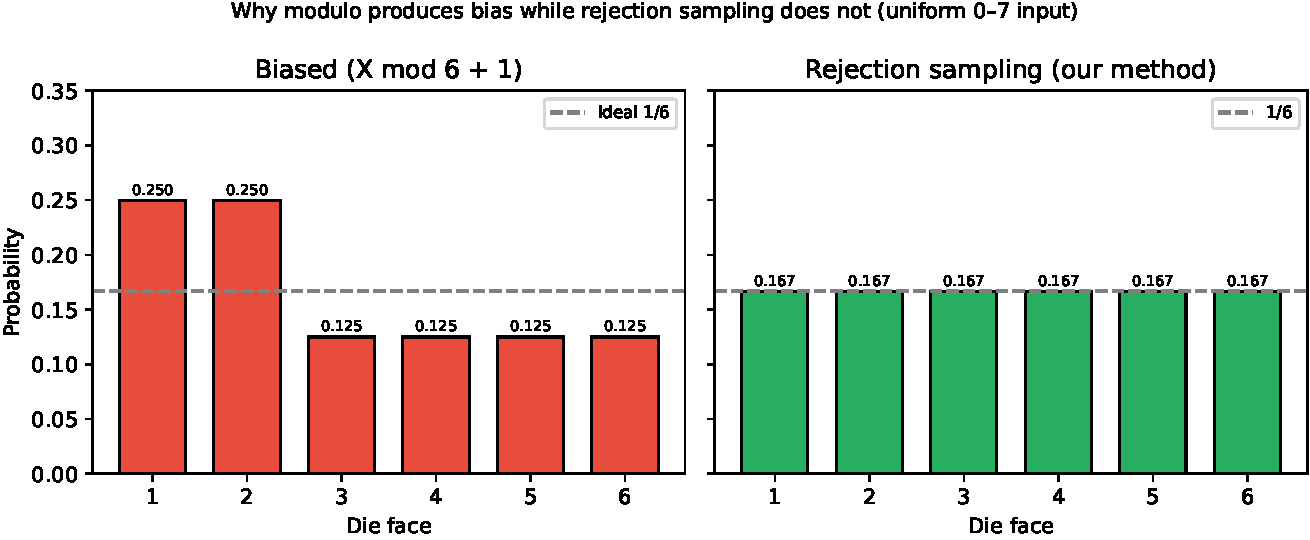
\includegraphics[width=0.98\linewidth]{figures/modulo-vs-rejection-bars.pdf}
\caption{Comparison of the biased modulo mapping with the exactly uniform distribution obtained by rejection sampling. Both start from a uniform random variable on $\{0,\dots,7\}$.}
\label{fig:bias}
\end{figure}

The rejection rule is realised in a few lines of classical post-processing after measurement; see the \texttt{pick\_valid\_dice} routine in the accompanying implementation.

\section{Two Dice and Independence}
\label{sec:two}

Tavla (and standard backgammon) requires two independent dice. We encode both dice in a single six-qubit circuit:
\[
|\Psi\rangle = H^{\otimes 6}|000000\rangle = \frac{1}{8}\sum_{x=0}^{7}\sum_{y=0}^{7}|x\rangle|y\rangle.
\]
The first three qubits represent die 1 and the second three represent die 2. Because the state is a tensor product, the two registers are independent even before measurement. After applying the per-die rejection rule we obtain a pair $(D_1,D_2)$ whose joint distribution is exactly uniform over the $6\times 6$ grid.

\begin{proposition}[Joint uniformity of two dice]\label{prop:joint}
Let $D_1=X\mid X\in A$ and $D_2=Y\mid Y\in A$. Then for every $i,j\in A$,
\[
P(D_1=i,D_2=j)=\frac{1}{36}.
\]
\end{proposition}

\begin{proof}
The six-qubit state factors, therefore $X$ and $Y$ are independent and each uniform on $\{0,\dots,7\}$. The event that both lie in $A$ has probability $(6/8)^2=9/16$. The conditional probability of any particular ordered pair is therefore
\[
\frac{(1/64)}{(36/64)}=\frac{1}{36}.
\]
\end{proof}

\section{Generalisation and Batch Success Probability}

For $m$ dice the circuit uses $3m$ qubits and the per-shot acceptance probability is
\[
p_m = \Bigl(\frac{6}{8}\Bigr)^m = \Bigl(\frac{3}{4}\Bigr)^m.
\]
The expected number of shots until the first valid $m$-tuple is $\mathbb{E}[T_m]=1/p_m=(4/3)^m$. For the two-dice case of interest, $\mathbb{E}[T_2]=16/9\approx 1.78$ raw shots (well below the batch size of 64 used in production). The probability that a complete batch of $B=64$ shots contains \emph{no} valid pair is
\[
(1-p_2)^{64}=\Bigl(\frac{7}{16}\Bigr)^{64}\approx 1.5\times 10^{-23},
\]
which is negligible for all practical purposes.

\section{Algorithm}

The end-to-end procedure executed by the service (identical for Aer and IBM) is:

\begin{verbatim}
Input: m (dice), B (shots per batch, default 64)
n <- 3 * m
Build n-qubit circuit, n classical bits
Apply H to every qubit
Measure every qubit
for up to 4 batches:
    run circuit for B shots (memory=True)
    for each bitstring in result memory:
        decode m groups of 3 bits -> integers in 0..7
        if all integers are in 1..6:
            return the m-tuple as dice
return secure classical fallback (last resort)
\end{verbatim}

The quantum portion is a single layer of $3m$ Hadamard gates followed by $3m$ single-qubit measurements (gate depth $1$ in the ideal parallel model; the measurement adds one further layer). Classical post-processing per batch costs $O(Bm)$, and for $m=2$ a single batch of $64$ shots almost always suffices.

\section{Service Architecture and Contract}
\label{sec:arch}

The quantum sampling layer is deliberately isolated from the game engine. A lightweight FastAPI micro-service exposes a single endpoint
\[
\texttt{GET /roll?backend=aer|ibm\&dice=2}.
\]
The response always contains the classical values `d1`, `d2`, the actual backend that served the result, a job identifier, the number of shots consumed, and a Boolean `fallback` flag. When the client requests the IBM backend but the job times out or the hardware is unavailable, the service transparently returns an Aer result with \texttt{fallback=true}; a final last-resort path uses a classical cryptographic RNG. Consequently a roll requested as ``quantum'' may in practice be served by the simulator or by a classical generator: the explicit \texttt{backend} and \texttt{fallback} fields make this provenance auditable, but a genuine quantum-hardware origin is best-effort, not guaranteed. The Android game engine never sees quantum state vectors; it receives ordinary integers that are fed directly into the classical Tavla transition function.

Figure~\ref{fig:arch} depicts the data flow and the mathematical invariant that is preserved across both back-ends.

\begin{figure}[tbp]
\centering
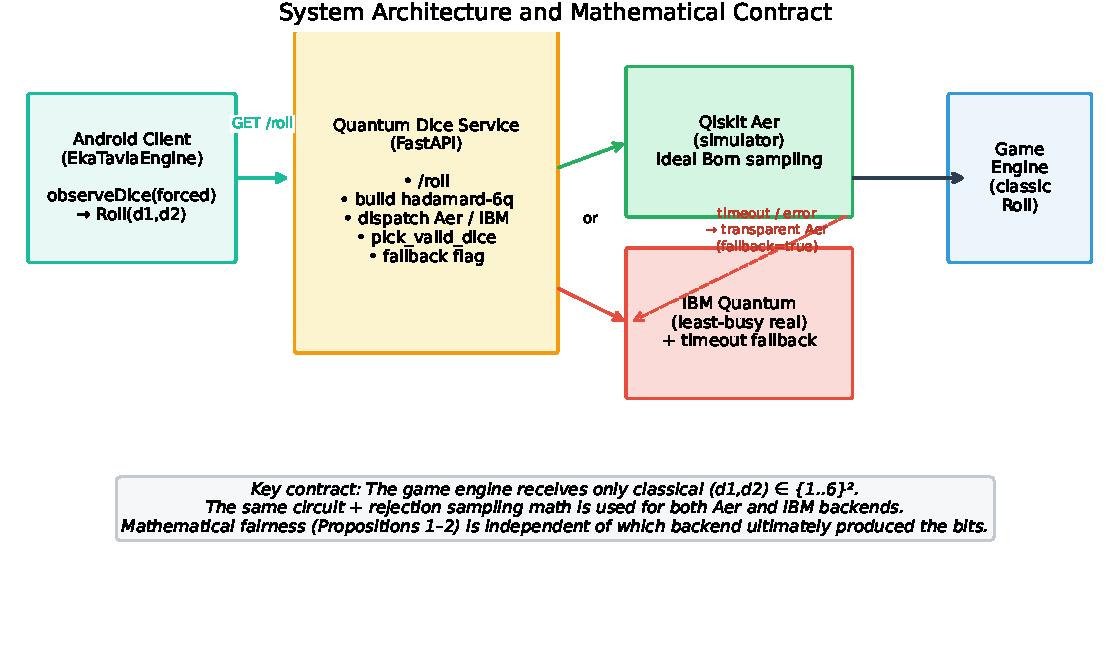
\includegraphics[width=0.98\linewidth]{figures/backend-contract.pdf}
\caption{Service architecture. The identical `hadamard-6q` circuit and rejection-sampling post-processor are used for both simulator and real hardware. The game engine receives only classical die values together with provenance metadata.}
\label{fig:arch}
\end{figure}

\section{Experimental Validation}
\label{sec:exp}

All experiments use the exact production circuit (\texttt{build\_dice\_circuit}) and the same accept test as the production \texttt{pick\_valid\_dice}; the run is seeded (\texttt{seed\_simulator}$=42$) and is therefore bit-for-bit reproducible from the accompanying scripts. We collected $N=50{,}000$ valid two-dice rolls on the Qiskit Aer simulator~\cite{qiskit2024}, corresponding to $100{,}000$ individual die faces.

\subsection{Marginal uniformity}

The observed face counts were
\[
(16521,16600,16783,16701,16446,16949).
\]
A $\chi^2$ goodness-of-fit test ($5$ degrees of freedom, no estimated parameters) against the uniform expectation of $16{,}666.67$ per face yields
\[
\chi^2=10.13,\qquad p=0.072,\qquad \mathrm{TVD}=0.0043.
\]
The test does not reject uniformity at the $5\%$ level; the largest single-face residual is $+282$ (about $2.4\sigma$). Because the Aer simulator draws from precisely the Born distribution that Propositions~\ref{prop:single}--\ref{prop:joint} already guarantee, this experiment is best read as a sanity check on the (pseudo-random) sampling and bit-decoding pipeline, not as an empirical test of fairness on a physical device; a high $p$-value is failure to reject, not positive confirmation. Figure~\ref{fig:obs} shows the observed versus expected counts.

\begin{figure}[tbp]
\centering
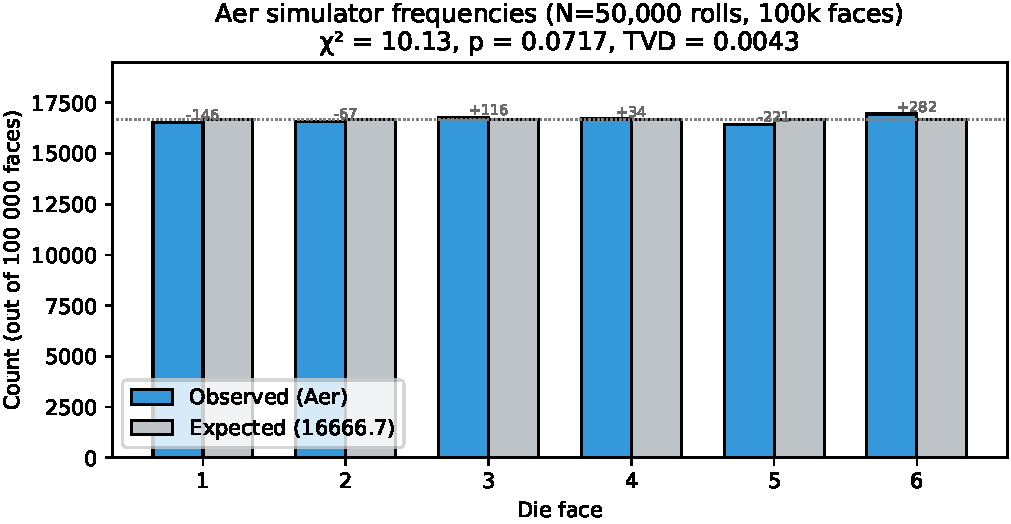
\includegraphics[width=0.95\linewidth]{figures/aer-observed-frequencies.pdf}
\caption{Observed face frequencies from 50{,}000 Aer rolls (100{,}000 die faces). Residuals are at the level of statistical fluctuation; the $\chi^2$ test does not reject uniformity.}
\label{fig:obs}
\end{figure}

\subsection{Joint uniformity}

The $6\times 6$ contingency table of $(d_1,d_2)$ pairs was tested for joint uniformity over the $36$ cells. The $\chi^2$ statistic on $35$ degrees of freedom is $26.85$ with $p=0.84$ and total-variation distance $0.0097$ from the ideal $1/36$ per cell, again consistent with the predicted distribution. We stress that independence of the two dice holds \emph{a priori} from the tensor-product structure of $|\Psi\rangle$ (Section~\ref{sec:two}); this table is therefore a joint-uniformity goodness-of-fit check, not an empirical independence test, and on an ideal simulator it cannot reveal the qubit crosstalk that a real device might exhibit.

\subsection{Acceptance rate}

Direct sampling of 200{,}000 raw shots produced 112{,}687 valid pairs, giving an empirical per-shot acceptance probability of $0.56344$, in close agreement with the theoretical value $(6/8)^2=0.5625$. The $50{,}000$ analysed rolls are the first $50{,}000$ accepted pairs of this same seeded run; returning the first accepted shot of a batch is unbiased because the raw shots are independent and identically distributed, so conditioning on ``first accepted'' preserves the uniform conditional law. With the production batch size $B=64$ the expected number of raw shots per valid pair is $\mathbb{E}[T_2]=16/9\approx 1.78$, and the probability that a batch contains no valid pair is $(7/16)^{64}\approx 10^{-23}$ (Section~\ref{sec:two}).

\subsection{Preliminary hardware run}
\label{sec:hw}

To probe how the ideal-circuit guarantee degrades on a physical device, we executed the identical \texttt{hadamard-6q} circuit once on the least-busy IBM Quantum processor available to us, \texttt{ibm\_marrakesh} (a 156-qubit Heron device), with $4000$ shots ($8000$ raw die values, job \texttt{d8gedtc2upec739jlc4g}). This is a single-run, single-backend measurement, intended as an honest illustration rather than a systematic characterisation.

The raw $0$--$7$ outcome distribution showed a small but clear readout-induced bias: total-variation distance $\mathrm{TVD}=0.0102$ from the ideal $1/8$, with a mild monotone trend (low values slightly suppressed, high values slightly enhanced). After the per-die rejection rule the conditioned face counts were $(720,706,741,771,779,783)$, giving $\chi^2=7.05$ ($5$ d.o.f., $p=0.22$) and $\mathrm{TVD}=0.0184$ from the ideal $1/6$---roughly four times the simulator residual ($0.0043$). The empirical per-shot acceptance was $0.5625$, matching the theoretical $9/16$. Figure~\ref{fig:ibm} compares both distributions to the ideal.

Two points follow. First, rejection sampling removes the \emph{structural} modulo bias but, as the Discussion (Section~\ref{sec:disc}) notes, it cannot remove \emph{hardware} bias: any skew already present in the raw $0$--$7$ samples is inherited by the conditional distribution---indeed the conditioned $\mathrm{TVD}$ here slightly exceeds the raw one. Second, even on a current device the residual unfairness is at the percent level and does not reject uniformity at the $5\%$ level for this sample size; nonetheless a deployment that advertises ``quantum dice'' should publish per-backend calibration rather than rely on the ideal guarantee. A systematic multi-backend study with readout-error mitigation and repeated runs is left to future work.

\begin{figure}[tbp]
\centering
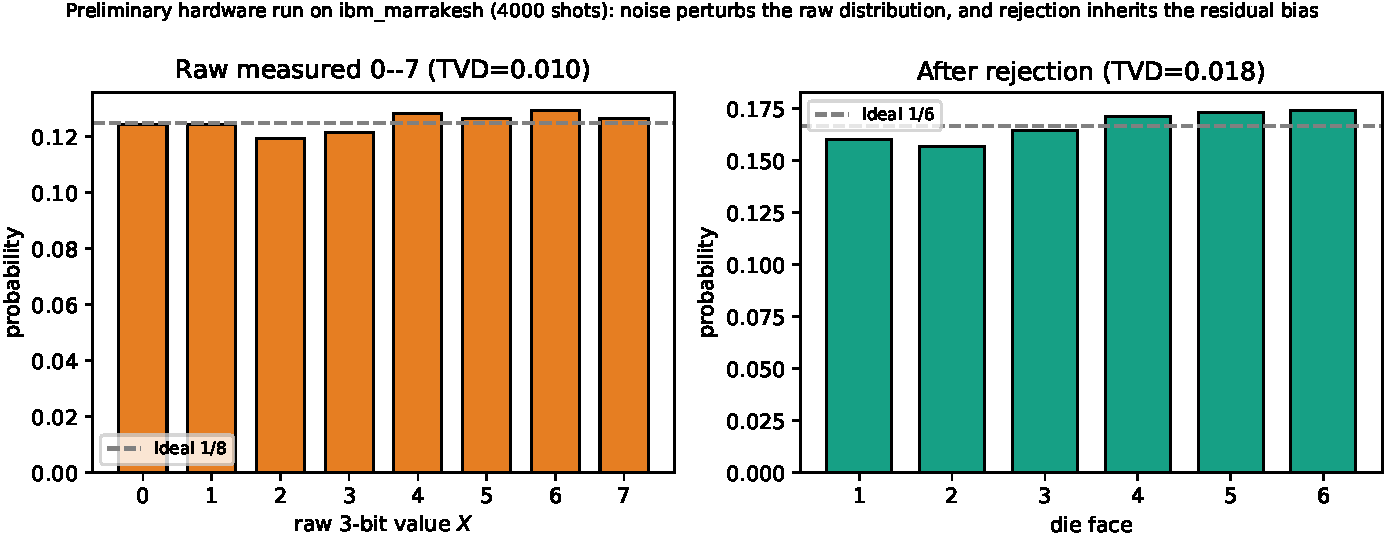
\includegraphics[width=0.98\linewidth]{figures/ibm-vs-ideal.pdf}
\caption{Preliminary single-run hardware result on \texttt{ibm\_marrakesh} ($4000$ shots). Left: the raw measured $0$--$7$ distribution shows readout-induced bias ($\mathrm{TVD}=0.0102$ from $1/8$). Right: after rejection, the conditioned $1$--$6$ die distribution has $\mathrm{TVD}=0.0184$ from $1/6$. Rejection removes the structural modulo bias but inherits the residual hardware bias.}
\label{fig:ibm}
\end{figure}

The circuit diagram actually executed is shown in Figure~\ref{fig:circuit}; the rejection flow is illustrated in Figure~\ref{fig:flow}.

\begin{figure}[tbp]
\centering
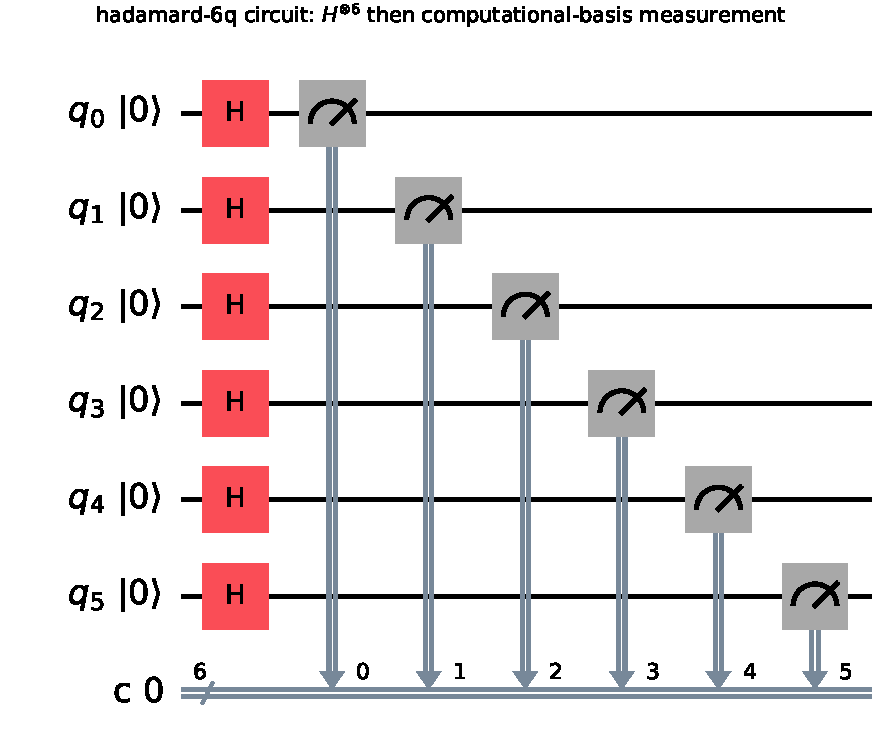
\includegraphics[width=0.98\linewidth]{figures/hadamard-6q-circuit.pdf}
\caption{The six-qubit circuit \texttt{hadamard-6q} used for every roll: six Hadamard gates followed by six computational-basis measurements (the classical register is bundled). Qubits $q_0$--$q_2$ encode die~1 and $q_3$--$q_5$ encode die~2; classical post-processing performs the per-die rejection test.}
\label{fig:circuit}
\end{figure}

\begin{figure}[tbp]
\centering
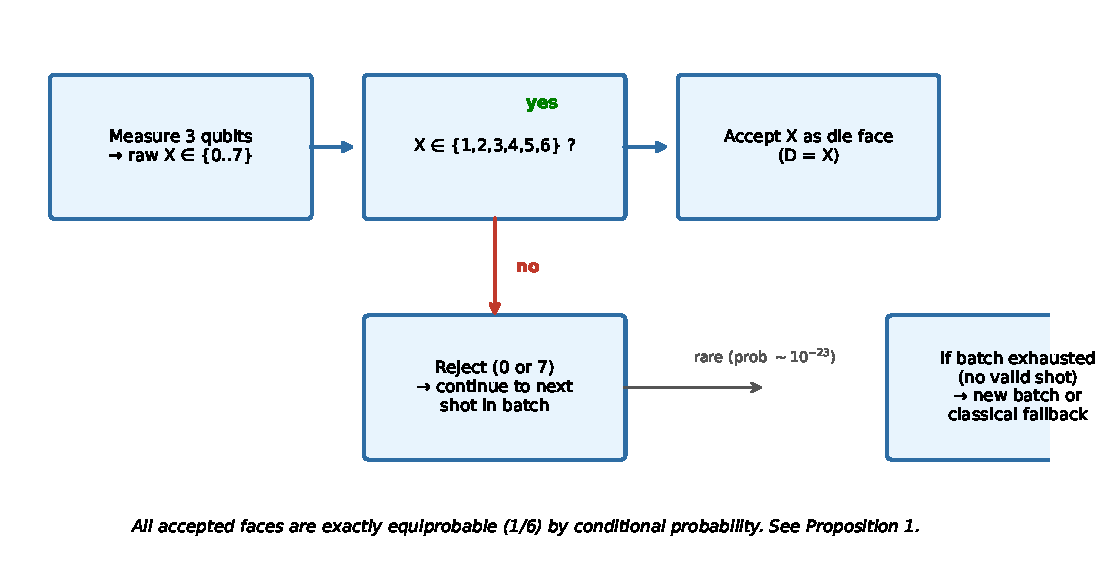
\includegraphics[width=0.92\linewidth]{figures/rejection-sampling-flow.pdf}
\caption{Rejection sampling decision flow for a single shot. The only quantum operation is the uniform superposition and measurement; the accept/reject test is classical and extremely cheap.}
\label{fig:flow}
\end{figure}

\section{Discussion}
\label{sec:disc}

The mathematical fairness guarantee holds only for the ideal circuit. On real IBM hardware, readout errors, decoherence, and gate infidelity will perturb the raw $0$--$7$ distribution before rejection. Because rejection discards two out of eight outcomes, any bias already present in the hardware samples is inherited by the conditional distribution (measured in Section~\ref{sec:hw}: $\mathrm{TVD}\approx 0.018$ on \texttt{ibm\_marrakesh}). Consequently, production deployments that advertise ``quantum dice'' should either (a) remain on the simulator, (b) publish per-backend calibration data together with the observed TVD, or (c) apply additional classical conditioning/extraction. In our service the `backend` and `fallback` fields make the provenance of every roll explicit, allowing downstream auditing.

From a systems perspective the construction is deliberately over-engineered for a mobile game: a remote round-trip, possible queueing, and quota consumption are all incurred for randomness that a modern phone can generate locally at essentially zero cost and with cryptographic strength. The value of the present work therefore lies less in ``better dice'' than in (i) a clean pedagogical example of mapping a continuous quantum probability distribution onto a discrete uniform one, (ii) a concrete, reproducible demonstration of cloud quantum computing inside a consumer application, and (iii) an existence proof that the engineering surface between a quantum backend and a classical game engine can be reduced to a few dozen lines of well-specified code.

Future extensions could include device-independent certified randomness protocols, on-device quantum simulators for zero-latency play, or generalisation to other dice geometries (e.g., 4-, 8-, 10-, 12-, 20-sided) with optimal qubit counts and minimal rejection overhead.

\paragraph{Limitations.} Three limitations bound the present claims. (i) All reported statistics are from the Aer simulator; we have not benchmarked real IBM hardware, where readout and gate noise perturb the raw $0$--$7$ distribution and where qubit crosstalk could induce the inter-die correlation that the product-state argument assumes away. (ii) The exactness result concerns the ideal circuit; under the fallback path a roll may be served by the simulator or a classical RNG, so end-to-end ``quantum'' provenance is best-effort. (iii) The contribution is a clean engineering-and-pedagogy construction rather than a new quantum primitive---for ordinary play a local CSPRNG is cheaper and cryptographically stronger, and the method provides no randomness \emph{certification} in the device-independent sense.

\section{Conclusion}

We have shown that a single-layer Hadamard circuit on three qubits per die, followed by the rejection of two out of eight measurement outcomes, yields a mathematically exact uniform six-sided die. The construction extends without modification to any number of independent dice via a product state. Reproducible simulator experiments are consistent with the predicted statistics, with the caveat that an ideal simulator validates the sampling pipeline rather than the fairness guarantee itself. By exposing the sampler through a narrow, auditable HTTP contract we separate the quantum sampling concern from the classical game logic; the same contract also carries hardware-sourced bits, and a preliminary run on \texttt{ibm\_marrakesh} confirms that the guarantee degrades gracefully (percent-level bias) under device noise; a systematic multi-device characterisation remains future work.

The implementation, the seeded experimental data, the generation scripts, and the figure sources are included in the repository~\cite{projectrepo}; the seeded run makes every reported number reproducible bit-for-bit.

\section*{Acknowledgements}

We thank the Qiskit open-source community; the Aer simulator made the reproducible experimental campaign straightforward, and the IBM Quantum Runtime primitives underpin the (not-yet-benchmarked) hardware path. The Android client and 3-D tabletop visualisation layers of Quantum Eka Tavla are outside the scope of this paper but provided the original motivation for a verifiable dice source.

\bibliographystyle{plain}
\bibliography{references}

\end{document}
